\documentclass{beamer}
\usepackage[utf8]{inputenc}
\usepackage{graphicx}
\graphicspath{ {./images/} }

\usetheme{Madrid}
\useoutertheme{miniframes}
\useinnertheme{circles}

\definecolor{UBCblue}{rgb}{0.04706, 0.13725, 0.26667}

\usecolortheme[named=UBCblue]{structure}

\author[Jayashre]{Jayashre}
\title[SecureDash]{SecureDash}
\subtitle{Advancing Smart Grid Security with an Intrusion Detection Framework}
\titlegraphic{
\includegraphics[width=2.3cm]{securedash.png}}
\institute{Project Overview and Development}
\date{\today}

\setbeamertemplate{footline}{
  \leavevmode%
  \hbox{%
    \begin{beamercolorbox}[wd=.3\paperwidth,ht=2.25ex,dp=1ex,left,center]{author in head/foot}%
      \usebeamerfont{author in head/foot}\hspace*{0.5cm}\insertshortauthor\hspace*{0.5cm}
    \end{beamercolorbox}%
    \begin{beamercolorbox}[wd=.4\paperwidth,ht=2.25ex,dp=1ex,center]{title in head/foot}%
      \usebeamerfont{title in head/foot}\insertshorttitle
    \end{beamercolorbox}%
    \begin{beamercolorbox}[wd=.3\paperwidth,ht=2.25ex,dp=1ex,right,center]{date in head/foot}%
      \usebeamerfont{date in head/foot}\hspace*{0.5cm}\insertframenumber{} / \inserttotalframenumber\hspace*{0.5cm}
    \end{beamercolorbox}}%
  \vskip0pt%
}

\setbeamertemplate{headline}{}

%\logo{
\includegraphics[height=1cm]{images/securedash.png}}

\AtBeginSection[]
{
  \begin{frame}
    \frametitle{Table of Contents}
    \tableofcontents[currentsection]
  \end{frame}
}
%------------------------------------------------------------


\begin{document}

\frame{\titlepage}

\begin{frame}
\frametitle{Table of Contents}
\tableofcontents
\end{frame}
%---------------------------------------------------------


\section{Project Overview}
\begin{frame}{Project Overview}
\par This project aims to enhance Smart Grid security by developing an advanced intrusion detection system that leverages machine learning to combat cyber threats, such as DDoS attacks. The primary goal is to advance intrusion detection capabilities within smart energy grids, ensuring uninterrupted operation and safety in our increasingly digital world. By integrating real-time monitoring, advanced anomaly detection, and robust threat mitigation strategies, the project seeks to protect critical infrastructure from evolving cyber threats and maintain the reliability and resilience of modern energy grids.
\end{frame}

\section{What is Smart Grid and Intrusion Detection System (IDS)?}

\begin{frame}{Smart Grid \& Intrusion Detection System}
\begin{minipage}{0.6\textwidth}
\textbf{Smart Grid:} An advanced electricity network utilizing digital communication technology for efficient and reliable electricity and data management. It enables two-way communication, optimizing resource utilization, incorporating renewable energy sources, and enhancing grid resilience through real-time monitoring and control.
\par \textbf{IDS in Smart Grid:} Safeguards the communication network against cyber threats by continuously detecting both known and unknown attacks across different layers: Home Area Network (HAN) for individual homes, Neighborhood Area Network (NAN) for aggregating data, and Wide Area Network (WAN) for the larger infrastructure.
\end{minipage}%
\begin{minipage}{0.4\textwidth}
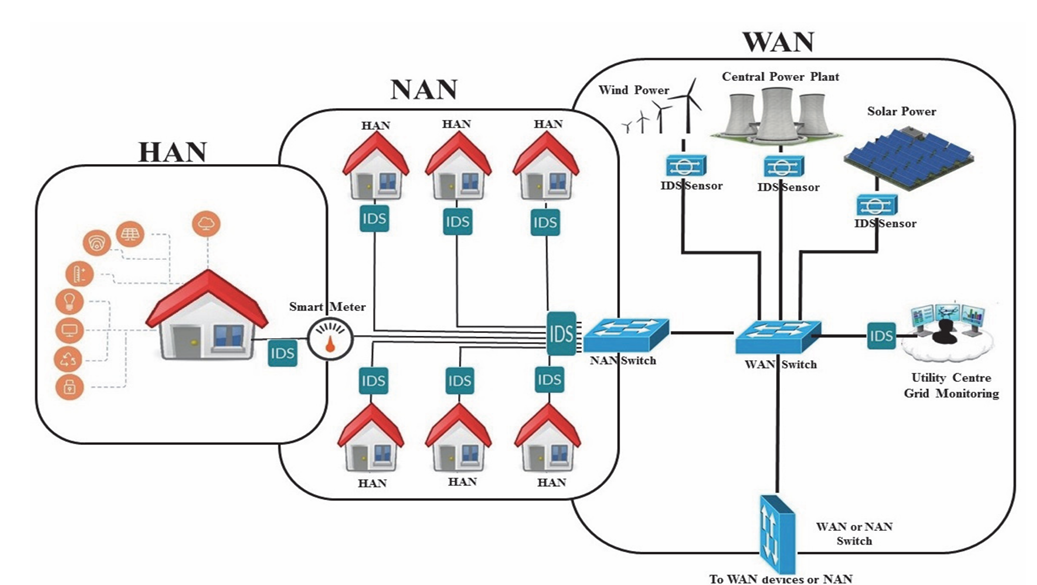
\includegraphics[width=\textwidth]{images/arch.png}
\end{minipage}
\end{frame}

\section{Tech Stack}

\begin{frame}{Tech Stack}
\textbf{Technologies Used}
\begin{enumerate}
    \item \textbf{Python}: For implementing machine learning and deep learning models.
    \item \textbf{Google Colab}: For the development of machine learning models in Python.
    \item \textbf{Scapy \& Numpy}: For capturing and processing network packets.
    \item \textbf{Standard Scaler \& ADASYN}: For data scaling and handling class imbalance.
    \item \textbf{MySQL}: For backend database management.
    \item \textbf{Power BI}: For real-time visualization and analytics.
    \item \textbf{Electron, HTML, CSS \& Javascript}: : For developing the desktop application.
    \item \textbf{Flask}: For running the web server to view the database.
\end{enumerate}
\end{frame}

\section{Machine Learning Model Development}

\begin{frame}{Machine Learning Model Development}
\begin{enumerate}
    \item \textbf{Hybrid Deep Learning Model}: Combines Convolutional Neural Network (CNN) and Gated recurrent unit (GRU) for effective feature extraction and sequence learning.
    \item \textbf{Data Preprocessing}: Features scaled using Standard Scaler, and class imbalance addressed with ADASYN.
    \item \textbf{Model Architecture}
    \begin{itemize}
        \item \textbf{CNN} for feature extraction.
        \item \textbf{GRU} for capturing long-term dependencies
        \item \textbf{Flattening} CNN Layer for Feature Integration
        \item \textbf{Concatenation} Layer for Merging Outputs from CNN and GRU
        \item Addition of \textbf{Fully Connected} Layer
        \item \textbf{Dropout Layer} to Prevent \textit{Overfitting}
        \item \textbf{SoftMax Layer} for \textit{Classification}
    \end{itemize}
    \item \textbf{Training}: The model was trained on the \href{https://www.unb.ca/cic/datasets/ddos-2019.html}{\textbf{CIC-DDOS2019}} dataset.
\end{enumerate}
\end{frame}


\end{document}